\documentclass[12pt]{exam}
\usepackage[utf8]{inputenc}
\usepackage{amsmath,amstext,amsthm,amssymb,amsxtra, graphicx,cancel}
\usepackage[top=1.5in, bottom=1.5in, left=1.25in, right=1.25in]	{geometry}
%\usepackage[normalem]{ulem}
\usepackage{txfonts} % pxfonts txfonts 
\usepackage[T1]{fontenc}
\usepackage{lmodern}
\renewcommand*\familydefault{\sfdefault}
 \usepackage{euler}   % better than the option below
\usepackage{pdfsync}
\usepackage{multicol}
\newcommand{\ci}[1]{_{ {}_{\scriptstyle #1}}}
\graphicspath{ {images/} }


\newcommand{\norm}[1]{\ensuremath{\left\|#1\right\|}}
\newcommand{\abs}[1]{\ensuremath{\left\vert#1\right\vert}}
\newcommand{\ip}[2]{\ensuremath{\left\langle#1,#2\right\rangle}}
\newcommand{\p}{\ensuremath{\partial}}
\newcommand{\pr}{\mathcal{P}}

\newcommand{\pbar}{\ensuremath{\bar{\partial}}}
\newcommand{\db}{\overline\partial}
\newcommand{\D}{\mathbb{D}}
\newcommand{\B}{\mathbb{B}}
\newcommand{\Sp}{\mathbb{S}}
\newcommand{\T}{\mathbb{T}}
\newcommand{\R}{\mathbb{R}}
\newcommand{\Z}{\mathbb{Z}}
\newcommand{\C}{\mathbb{C}}
\newcommand{\N}{\mathbb{N}}
\newcommand{\Q}{\mathbb{Q}}
\newcommand{\mQ}{\mathcal{Q}}
\newcommand{\mS}{\mathcal{S}}
\newcommand{\scrH}{\mathcal{H}}
\newcommand{\scrL}{\mathcal{L}}
\newcommand{\td}{\widetilde\Delta}
\newcommand{\pw}{\text{PW}}
\newcommand{\esup}{\text{ess.sup}}
\newcommand{\Tn}{\mathcal{T}_n}
\newcommand{\Bn}{\mathbb{B}_n}
\newcommand{\rt}{\mathcal{O}}
\newcommand{\avg}[1]{\langle #1 \rangle}
\newcommand{\one}{\mathbbm{1}}
\newcommand{\eps}{\varepsilon}
\newcommand{\grad}{\nabla}

\newcommand{\La}{\langle }
\newcommand{\Ra}{\rangle }
\newcommand{\rk}{\operatorname{rk}}
\newcommand{\card}{\operatorname{card}}
\newcommand{\ran}{\operatorname{Ran}}
\newcommand{\osc}{\operatorname{OSC}}
\newcommand{\im}{\operatorname{Im}}
\newcommand{\re}{\operatorname{Re}}
\newcommand{\tr}{\operatorname{tr}}
\newcommand{\vf}{\varphi}
\newcommand{\f}[2]{\ensuremath{\frac{#1}{#2}}}

\newcommand{\kzp}{k_z^{(p,\alpha)}}
\newcommand{\klp}{k_{\lambda_i}^{(p,\alpha)}}
\newcommand{\TTp}{\mathcal{T}_p}
\newcommand{\m}[1]{\mathcal{#1}}
\newcommand{\md}{\mathcal{D}}
\newcommand{\qan}{\abs{Q}^{\alpha/n}}
\newcommand{\sbump}[2]{[[ #1,#2 ]]}
\newcommand{\mbump}[2]{\lceil #1,#2 \rceil}
\newcommand{\cbump}[2]{\lfloor #1,#2 \rfloor}

\newcommand{\hn}{{1}}
\newcommand{\dd}{{08-31}}
\newcommand{\class}{Aero 321}
\newcommand{\term}{Fall 2023}
\newcommand{\examnum}{Homework \hn: Due \dd}
\newcommand{\examdate}{}
\newcommand{\timelimit}{75 Minutes}
\newcommand{\vc}[3]{\langle #1,#2,#3\rangle}
\newcommand*{\vv}[1]{\vec{\mkern0mu#1}}
\newcommand{\bv}[1]{\boldsymbol{#1}}
\newcommand{\hide}[1]{}
\newcommand{\uvec}[1]{\boldsymbol{\hat{\textbf{#1}}}}
\newcommand{\vex}[1]{\boldsymbol{{\textbf{#1}}}}
\newcommand{\px}{\frac{\partial}{\partial x}}
\newcommand{\py}{\frac{\partial}{\partial y}}
\newcommand{\pt}{\frac{\partial}{\partial t}}
\newcommand{\pxx}{\frac{\partial^2}{\partial x^2}}
\newcommand{\pyy}{\frac{\partial^2}{\partial y^2}}
\newcommand{\ptt}{\frac{\partial^2}{\partial t^2}}


\pagestyle{head}
\firstpageheader{}{}{}
\runningheader{\class}{ Page \thepage\ of \numpages}{\examnum}
\runningheadrule

\makeatletter
\renewcommand*\env@matrix[1][*\c@MaxMatrixCols c]{%
  \hskip -\arraycolsep
  \let\@ifnextchar\new@ifnextchar
  \array{#1}}
\makeatother

\printanswers
\begin{document}

\noindent
\begin{tabular*}{\textwidth}{l @{\extracolsep{\fill}} r @{\extracolsep{6pt}} l}
\textbf{\class} & \textbf{Name:} & \makebox[2in]{\bf{Benjamin Tollison}}\\
\end{tabular*}\\
\rule[2ex]{\textwidth}{2pt}
%
\begin{questions}
\begin{question}
A small satellite has six thrusters, each capable of applying F units of force (if used).
The thrust directions and thruster locations (in a centroidal body-fixed coordinate system)
are provided in the table. 

Write a relationship between the thrust on-off selector vector and the net force and
moment produced using a Ax = b system of equations.
\end{question}
\begin{solutionorbox}[\stretch{1}]
\\
a)\\
The way that I approach this problem is that I wanted the first row in \(\vec{b}\) to be \(\sum{F_x}\) and 
the second and third to be \(\sum{F_y}\) and \(\sum{F_z}\).
Therefore \(a_{11} = F_{thruster 1} \hat{x}\) and etc. 
Which ended up being the transpose of the thrust direction matrix given that we set the thrust equal to 1.
\\
To find the 3 summations of the moments I was going to use the equation \(M = \vec{r} \times \vec{F}\),
but for each thruster and each force vector I ignored the appropriate columns when taking the cross product. Such as
\(M_x = (\cancelto{0}{r_x},r_y,r_z) \times (\cancelto{0}{F_x},F_y,F_z)\) and therefore building the following A matrix.
\[ A =
\begin{bmatrix}
  -1. & 0. & 0. & 0. & 0. & 1.\\
  0. & 1. & 0. & -1. & 0. & 0.\\
  0. & 0. & 1. & 0. & -1. & 0.\\
  0. & 8. & -8. & 8. & -8. & 0.\\
  -8. & 0. & 8. & 0. & 8. & -8.\\
  -8. & -8. & 0. & -8. & 0. & -8.
\end{bmatrix}
\]
b) \\
In order to find the sum of forces and moments when the 1,2,5 are all firing, we just have to set 
\[ \vec{x} = 
\begin{bmatrix}
  1 \\ 1 \\ 0 \\ 0 \\ 1 \\ 0
\end{bmatrix}
\]
and do \(A \cdot \vec{x}\) to find \(\vec{b}\) Which is
\[\vec{b} = \begin{bmatrix}
 -1. \\ 1. \\ -1. \\ 0. \\ 0. \\ -16 
\end{bmatrix}
\]
c)
To find all the 2 thruster combinations that only produce a moment, we can first define \[\vec{b} = \begin{bmatrix}
  0\\0\\0\\ \neq 0 \\ \neq 0 \\ \neq 0
\end{bmatrix}
\]
Then, I listed out all of the possible combinations of thrusters, which in total was 64, then I did \(A \cdot \vec{x}\) and filtered out all the combinations that don't meet the requirements for \(\vec{b}\).
The \(\vec{x}\) that met the requirements were (0, 0, 0, 0, 0, 0), (0, 0, 1, 0, 1, 0), (0, 1, 0, 1, 0, 0), (0, 1, 1, 1, 1, 0), (1, 0, 0, 0, 0, 1), (1, 0, 1, 0, 1, 1), (1, 1, 0, 1, 0, 1), (1, 1, 1, 1, 1, 1)
\\
\\
\(\therefore\) the thruster pairs (3,5), (2,4), and (1,6)
\end{solutionorbox}

\newpage 
\begin{question}
A system is modeled by the ode: \(\ddot{x} = -\dot{x} - x + \sin \omega t\); \(x(0) = x_0\) and \(\dot{x}(0) = \dot{x}_0\). The input
frequency is \(\omega\) (rad/sec) and the output is x(t) \\
i) Write the form fo the homogeneous solution \\
ii) Determind the particular solution \\
iii) Take the limit of x(t) as t->\(\infty\) and see if the particular solution remains \\
\end{question}
\begin{solutionorbox}[\stretch{1}]
\[x(t) = x_h + x_p\]
i)
\[x_h = c e^{s(t-t_0)}\]
The characteristic equation is \(s^2 + s + 1 = 0\)
\[s = \frac{-1 \pm \sqrt{1-\cancelto{4}{4(1)(1)}}}{2(1)} = \frac{-1}{2} \pm i\frac{\sqrt{3}}{2}\]
Making the homogeneous equation \[x_h(t) = c_1 e^{t(\frac{-1}{2} - i\frac{\sqrt{3}}{2})} + c_2 e^{t(\frac{-1}{2} + i\frac{\sqrt{3}}{2})}\]
\[x_h(t) = c_1 \frac{e^{-t/2}}{\cos{\frac{t\sqrt{3}}{2}} + i \sin{t\frac{\sqrt{3}}{2}}} + c_2 e^{-t/2} \left[\cos{\frac{t\sqrt{3}}{2}}+  i \sin{t\frac{\sqrt{3}}{2}}\right]\]
ii)\\
The particular solution is going to be of the form \(x_p(t) = a \sin{\omega t} + b \cos{\omega t}\)
\[\dot{x}_p = a \omega \cos{\omega t} - b \omega \sin{\omega t}\]
\[\ddot{x}_p = -a \omega^2 \sin{\omega t} -b \omega^2 \cos{\omega t}\]
Plugging in the particular solution and its derivatives into the original equation produces the following
\[-a \omega^2 \sin{\omega t} -b \omega^2 \cos{\omega t} +
a \omega \cos{\omega t} - b \omega \sin{\omega t} +
a \sin{\omega t} + b \cos{\omega t} = \sin{\omega t} \]
\[\sin{\omega t} (-a\omega^2 - b\omega - a) + \cos{\omega t} (-b\omega^2 +a\omega -b) = \sin{\omega t}\]
Which produces the following system of equations:
\[
\begin{bmatrix}
-\omega^2-1 & -\omega\\
\omega & -\omega^2-1  
\end{bmatrix}
\begin{bmatrix}
a\\b 
\end{bmatrix}
= \begin{bmatrix}
1\\0 
\end{bmatrix}
\]
\[\Rightarrow a = \frac{-\omega^2 - 1}{\omega^4 + 3\omega^2 + 1}\]
\[\Rightarrow b = \frac{-\omega}{\omega^4 + 3\omega^2 + 1}\]
iii) \\
When you take the limit of the homogenous solution, \(x_h(\infty) = 0\) because the real part of s is negative making it a decaying function.
When you take the limit of the particular solution, the values will oscillate between the amplitudes dictated by a,b.
\[\therefore \lim_{t\rightarrow\infty} x(t) = \cancelto{0}{x_h} + x_p(t)\] 
\end{solutionorbox}


\newpage 
\begin{question}
Use the Euler integration scheme to obtain the numerical solution to the previous
problem over a time span of 30 sec, for the specific case of \(\omega= 1\) rad/sec, \(x(0)=1\) and \(\dot{x}(0)=1\). Choose the integration step size appropriately.
\end{question}
\begin{solutionorbox}[\stretch{1}]
\[
\begin{matrix}
x_1 = x\\
x_2 = \dot{x} \\
x_1(0) = x_0 = 1\\
x_2(0) = \dot{x}_0 = 1
\end{matrix}
\]
After applying the linearization we get the following system of equations
\[\begin{bmatrix}
\dot{x}_1 \\ \dot{x}_2  
\end{bmatrix}
=
\begin{bmatrix}
x_2 \\ \sin{\omega t} - x_2 + x_1  
\end{bmatrix}
\]
Applying 1st order taylor series approximation gives us the following
\[\begin{bmatrix}
x_{1,i+1} \\ x_{2,i+1}
\end{bmatrix} = \begin{bmatrix}
x_{1,i} + \Delta t x_{2,i+1} \\ x_{2,i} + \Delta t(\sin{\omega t_i}-x_{2,i+1} + x_{1,i+1})
\end{bmatrix}\]
Algerbriac simplification and putting into matrix form produces:
\[\begin{bmatrix}
1 & -\Delta t \\ -\Delta t & 1+\Delta t
\end{bmatrix}
\begin{bmatrix}
x_{1,i+1} \\ x_{2,i+1}
\end{bmatrix}
=
\begin{bmatrix}
x_{1,i} \\ x_{2,i} + \Delta t \sin{\omega t_i}  
\end{bmatrix}
\]
Solving for \(x_{1,i+1}\) and \(x_{2,i+1}\) with cramer's rule
\[x_{1,i+1} = \frac{x_{1,i}+\Delta t x_{1,i} + \Delta t x_{2,i} + \Delta t^2 \sin{\omega t_i}}{1+\Delta t + \Delta t^2}\]
\[x_{2,i+1} = \frac{x_{2,i}-\Delta t x_{1,i} + \Delta t \sin{\omega t_i}}{1+\Delta t + \Delta t^2}\]
\end{solutionorbox}
\pagebreak
Graphing the following with a step in time = 0.01 \\
\begin{figure}[h]
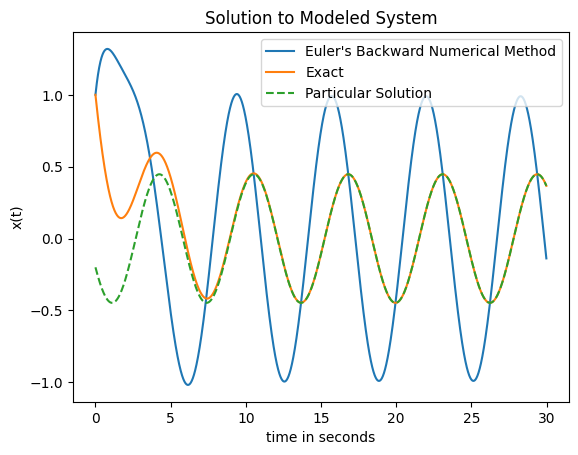
\includegraphics[width = \linewidth]{Comparing-solutions-graph.png}  
\centering
\end{figure}
ii) \\
The exact solution converges to the particular solution relatively fast on the time scale of 30s. 
The oscillation is maitained by the particular solution, and the amplitude is less than the intial disturbence.
The input and output phase are in sync, while the numerical solution is slightly out of sync.

\end{questions}
\end{document}
